\section{Polling window}
    To calculate a $\Delta$Q, we take all the outcome instances that ended within a window of time from $t_l$ to $t_u$, a lower and upper time bound.
    
    Suppose we are at time $t$, the window we will display is the  \textbf{window of time $(t-1)_{l}$ - $(t-1)_u$} with $t-1$ equal to $t - x$, and $x$ the polling rate. This is to account for various overheads that need to be taken into consideration, which could be network overhead, the wrapper overhead, C++ latency \dots Imagine multiple outcome instances that are ended at a time slightly lower but close to t, and due to the overheads the messages arrives at a time slightly higher but close to t, the outcome instance would not be taken into consideration for the calculation of a $\Delta$Q.
    
    \begin{figure}[H]
        \begin{center}
            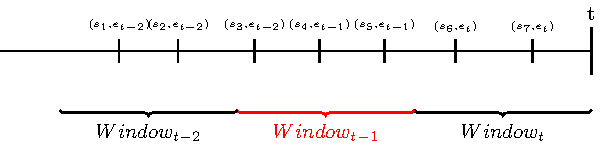
\includegraphics{tikz/window.pdf}
        \end{center}
    \end{figure}

    The polling window then advances every $x$ seconds setting the new window: 
    \begin{center}
        From: $(t-1)_l$, $(t-1)_u$ $\xrightarrow{t + 1}$ $t_l, t_u$. \\
        Where: $t_l = (t-1)_u$ and $t_u = (t-1)_u + x$ 
    \end{center}
